\documentclass[a4paper, 11pt]{article}

\usepackage[british]{babel}
\usepackage[autostyle]{csquotes}
\usepackage[colorlinks=true, urlcolor=blue, citecolor=blue]{hyperref}
\usepackage{graphicx}
\usepackage{float}
\usepackage{geometry}
\usepackage[ruled,vlined]{algorithm2e}

\graphicspath{{images/}}
\geometry{margin=2.0cm}

\begin{document}

\title{Machine Learning to Study Patterns in Chess Games}
\author{Student Number: 690065435}
\date{Academic Year 2022/2023}

\maketitle

\begin{abstract}
{Abstract here}.

\begin{center}
\end{center}
\end{abstract}

\vspace*{\fill}
\begin{center}

\vspace{1em}
I certify that all material in this report which is not my own work has been identified.
\end{center}
\vspace{1em}

Signature: \hrulefill

\newpage

\section{Introduction}

\section{Project Specification}

\section{Design}

\subsection{Data Pipeline}

\begin{figure}[h]
    \centering
    \caption{Data Pipeline Diagram for the Project}
    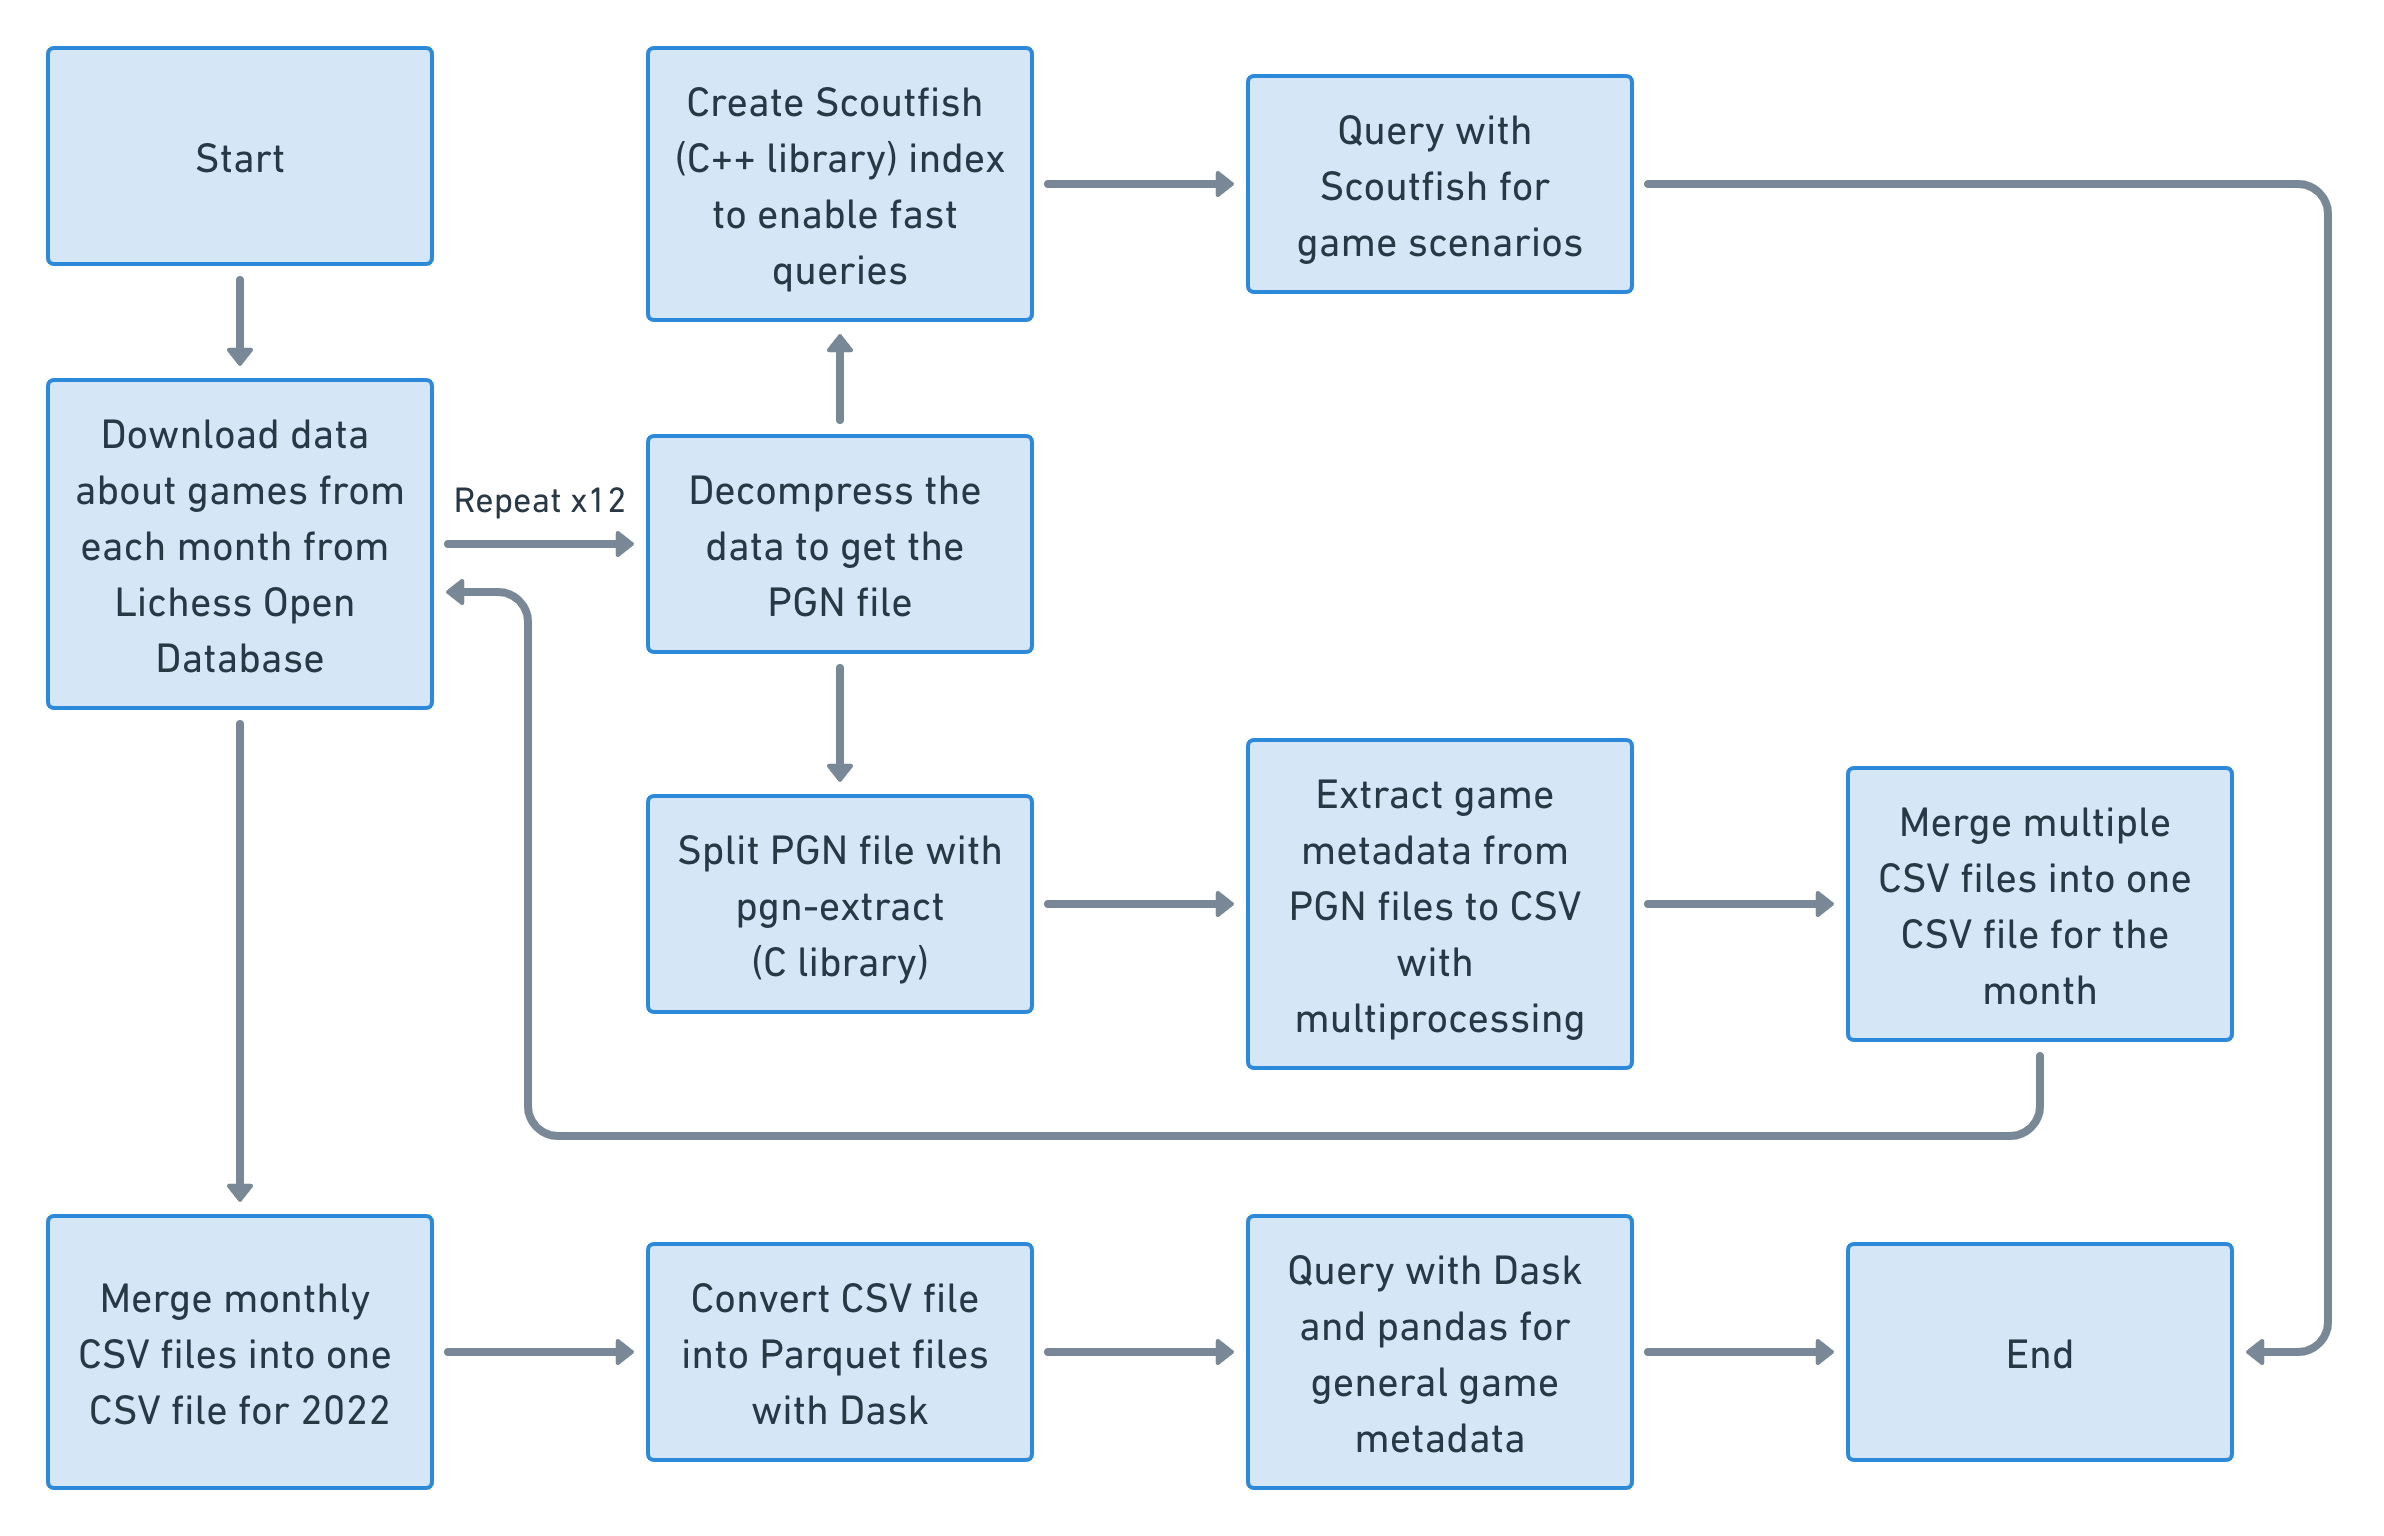
\includegraphics[width=0.8\textwidth]{Data Pipeline.png}
\end{figure}

Data processing was paramount to the success of my project -- it was important to use a large sample size to ensure that our insights represent the general population of chess games. I used the Lichess Open Database of standard rated games for my data source -- they upload tens of millions of games every month in PGN format, and they are easily accessible to the public. I decided to focus on games in 2022, as this enables me to capture the latest trends in chess.

\section{Development}

\section{Testing}

\section{Description of the Final Project}

\section{Evaluation of the Final Project}

\section{Critical Assessment of the Project}

\section{Conclusion}

\bibliography{main.bib}
\bibliographystyle{ieeetr.bst}

\end{document}